The core change is to the comparison weights, not to the one-sided test. D-SOS provides the inferential engine; the weighting step determines which observations participate in the comparison.

\paragraph{Setup.}
We observe source pairs $(x_i, s_i)_{i=1}^n$ and target pairs $(x'_j, t_j)_{j=1}^m$. Features $x$ carry the overlap structure---they determine which observations are comparable across groups. Each observation is mapped to a severity score where larger values mean worse behavior. The score need only preserve ranking; it need not be a calibrated probability or specific loss function.

Let $\overlap$ denote the common-support region where both groups place meaningful probability mass. The weighting scheme implicitly defines $\overlap$: an observation lies in $\overlap$ when both its source and target weights are non-negligible. Unweighted testing compares the observed populations directly. Source-weighted and target-weighted diagnostics downweight source-only or target-only regions. Doubly weighted testing asks whether the target is worse on $\overlap$ by applying both corrections simultaneously.

The null is the same across all four modes: the target is not substantively worse on the common support. Let $\Psi(Q_{\mathrm{src}}, Q_{\mathrm{tgt}})$ denote the one-sided harmful-shift functional from D-SOS, with larger values meaning a worse target. For each mode $m \in \{\mathrm{unw}, \mathrm{src}, \mathrm{tgt}, \mathrm{both}\}$, the empirical estimand is $\theta_m = \Psi(Q^{(m)}_{\mathrm{src}}, Q^{(m)}_{\mathrm{tgt}})$, where the superscript $(m)$ indicates whether that group's distribution is weighted.

\begin{figure}[t]
	\centering
	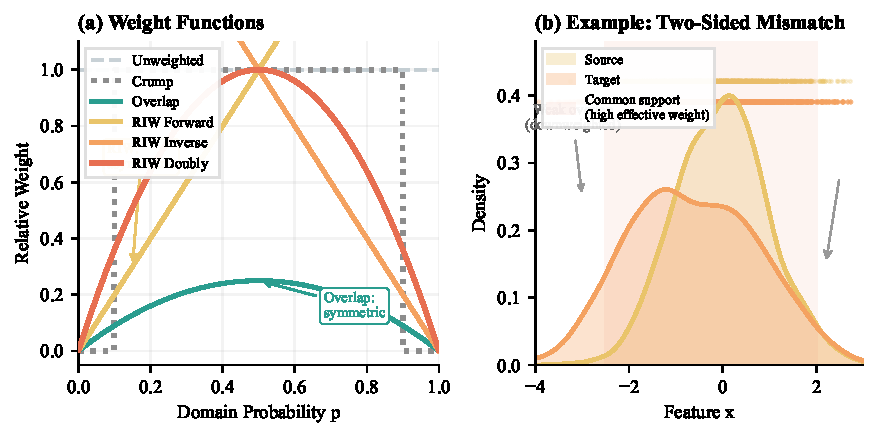
\includegraphics[width=0.98\linewidth]{figures/intro_reweighting_modes.pdf}
	\caption{Weighting modes for common-support testing. \textbf{(a)} Weight as a function of domain probability $p$ for six approaches: unweighted (uniform), Crump trimming (binary mask at threshold $\alpha=0.1$), overlap weights ($p(1-p)$), and stabilized RIW (forward, inverse, doubly weighted). Overlap weights are symmetric---the same function $w(p)$ applies to both groups---and reach zero at the boundaries. Stabilized RIW weights are asymmetric: forward (source) and inverse (target) corrections handle each group's density structure separately and remain bounded away from zero. \textbf{(b)} Concrete example with two-sided mismatch. Source and target densities overlap partially; weak-overlap regions on both tails carry non-comparable mass. The doubly weighted mode (both corrections active) concentrates effective weight on the common-support region (shaded), downweighting observations from low-overlap tails. The asymmetric corrections are what allow RIW to resolve two-sided contamination where symmetric schemes (overlap, Crump) cannot.}
	\label{fig:conceptual-weighting}
\end{figure}

\paragraph{Weights from domain probabilities.}
Let $\hat{p}(x) \in (0, 1)$ be the domain-classifier probability that an observation with features $x$ belongs to the target group, estimated held-out or out-of-bag. The density-ratio estimate is
\begin{equation}
  \hat{r}(x) = \frac{\hat{p}(x)}{1 - \hat{p}(x)} \cdot \frac{n}{m},
\end{equation}
where the prior ratio is inferred from group sizes~\cite{Bickel_2007}. A ratio $\hat{r}(x) > 1$ means the observation resembles a target; $\hat{r}(x) < 1$ means it resembles a source.

To stabilize raw ratio estimates under weak overlap, we use relative importance weighting~\cite{Yamada_2013}. For source-side correction,
\begin{equation}
  w_{\mathrm{source}}(x) = \frac{\hat{r}(x)}{(1 - \lambda) + \lambda \hat{r}(x)}.
\end{equation}
For target-side correction,
\begin{equation}
  w_{\mathrm{target}}(x) = \frac{1}{\lambda + (1 - \lambda) \hat{r}(x)}.
\end{equation}
The asymmetry is by design: $w_{\mathrm{source}}$ downweights source observations with $\hat{r}(x) \gg 1$ (those that look like targets), while $w_{\mathrm{target}}$ downweights target observations with $\hat{r}(x) \ll 1$ (those that look like sources). Only when both corrections are active together does the comparison restrict to the common support. Appendix Table~\ref{tab:weighting-benchmarks} provides a comprehensive comparison with overlap weights and Crump trimming.

The tuning parameter $\lambda \in [0, 1]$ controls the bias-variance trade-off. At $\lambda = 0$, weighting is strict density-ratio correction; at $\lambda = 1$, weights are uniform. Source-specific observations ($\hat{r}(x) \ll 1$) receive low source weight; target-specific observations ($\hat{r}(x) \gg 1$) receive low target weight. When both corrections are active, only observations plausible under both groups retain high weight.

\paragraph{Weighted score distributions.}
Let $\widehat{Q}_{\mathrm{src}}$ and $\widehat{Q}_{\mathrm{tgt}}$ denote the empirical score distributions. Weighted versions are defined by
\begin{equation}
  \mathbb{E}_{\widehat{Q}_{\mathrm{src},\lambda}}[g(S)] = \frac{\sum_{i=1}^n w_{\mathrm{source}}(x_i) g(s_i)}{\sum_{i=1}^n w_{\mathrm{source}}(x_i)}
\end{equation}
and
\begin{equation}
  \mathbb{E}_{\widehat{Q}_{\mathrm{tgt},\lambda}}[g(T)] = \frac{\sum_{j=1}^m w_{\mathrm{target}}(x'_j) g(t_j)}{\sum_{j=1}^m w_{\mathrm{target}}(x'_j)}.
\end{equation}
Within each active group, weights are normalized to sum to the group's sample size. The four empirical estimands become:
\begin{align}
  \theta_{\mathrm{unw}} &= \Psi(\widehat{Q}_{\mathrm{src}}, \widehat{Q}_{\mathrm{tgt}}), \\
  \theta_{\mathrm{src}} &= \Psi(\widehat{Q}_{\mathrm{src},\lambda}, \widehat{Q}_{\mathrm{tgt}}), \\
  \theta_{\mathrm{tgt}} &= \Psi(\widehat{Q}_{\mathrm{src}}, \widehat{Q}_{\mathrm{tgt},\lambda}), \\
  \theta_{\mathrm{both}} &= \Psi(\widehat{Q}_{\mathrm{src},\lambda}, \widehat{Q}_{\mathrm{tgt},\lambda}).
\end{align}
The doubly weighted estimand $\theta_{\mathrm{both}}$ is the primary object of this paper. Source-weighted and target-weighted variants serve as asymmetric diagnostics for one-sided mismatch; the unweighted test is the naive baseline.

\paragraph{Inference.}
The common-support correction applies to any score-based test for harmful shift that accepts per-observation weights. Estimate domain probabilities, set mode-specific weights, then run the one-sided test with permutation inference on weighted scores. The composition is specific to the Mann-Whitney functional: density-ratio weighting does not generically restrict a two-sample test to the common support, and the doubly weighted mode applies corrections to both arguments through a Hadamard-differentiable composition. Weighting changes which observations contribute to the test statistic; the null and permutation procedure are unchanged. The only new tuning parameter is $\lambda$, which influences the test through weight concentration and effective sample size.

In practice, use the doubly weighted test as the primary comparison; consult source-weighted or target-weighted variants to diagnose which side carries non-comparable observations. The effective sample size (below) provides a diagnostic for weight concentration. ESS and power trade off continuously across the $\lambda$ grid; lower $\lambda$ retains specificity but concentrates weights and reduces power. Practitioners should inspect the ESS diagnostic and the $\lambda$ sensitivity curve to balance false-alarm protection against power loss.

\paragraph{Formal properties.}
The doubly weighted estimand $\hat\theta_{\mathrm{both}}$ is an importance-weighted test statistic~\cite{pmlr-v161-bellot21b}: its balancing weights target a well-defined population quantity. Define the \emph{common-support score distributions} using the true density ratio $r(x) = p_T(x)/p_S(x)$:
\begin{align}
  \mathbb{E}_{Q_{\mathrm{src}}^{(r)}}[g(S)]
    &= \frac{\mathbb{E}_{P_S}[r(X)\,g(S)]}{\mathbb{E}_{P_S}[r(X)]}, \\
  \mathbb{E}_{Q_{\mathrm{tgt}}^{(1/r)}}[g(T)]
    &= \frac{\mathbb{E}_{P_T}[r(X)^{-1}\, g(T)]}{\mathbb{E}_{P_T}[r(X)^{-1}]},
\end{align}
for bounded measurable $g$. Both distributions concentrate on the common support $\overlap$, and the population target is
\begin{equation}
  \Theta = \Psi\!\left(Q_{\mathrm{src}}^{(r)},\; Q_{\mathrm{tgt}}^{(1/r)}\right).
\end{equation}

\begin{proposition}[Consistency]\label{prop:consistency}
Suppose $\hat{r} \to_p r$ in $L^2(P_S)$ and the score CDFs are absolutely continuous with bounded densities. For any fixed $\lambda \in [0, 1]$, $\hat\theta_{\mathrm{both}} \to_p \Theta_\lambda$ as $n, m \to \infty$, where $\Theta_\lambda$ is the population analog of $\hat\theta_{\mathrm{both}}$ with $\lambda$-interpolated weights. At $\lambda = 0$, $\Theta_0 = \Theta$.
\end{proposition}

\begin{proof}[Proof sketch]
The Mann-Whitney functional $\Psi$ is Hadamard differentiable under continuous score distributions~\cite{Kosorok_2008}, and the weighting transformation $Q \mapsto Q_\lambda$ is also Hadamard differentiable when $\hat{r} \to_p r$ in $L^2(P_S)$. By the functional delta method, the composition inherits differentiability, and consistency follows from the continuous mapping theorem. For $\lambda > 0$, bias relative to the $\lambda=0$ target is $O(1-\lambda)$. Details are in Appendix~\ref{app:theory}.
\end{proof}

\begin{proposition}[Permutation validity]\label{prop:permutation}
Let weights be estimated once from observed features $x$ and held fixed across all permutations. Under $H_0\colon \Theta \leq 0$, the permutation test that shuffles severity scores while holding weights fixed controls Type~I error conditionally on the weight configuration and therefore unconditionally at $\alpha$.
\end{proposition}

\begin{proof}[Proof sketch]
Domain-classifier probabilities depend only on features $x$, not on severity scores $s$, so weights are determined once $x$ is observed. Holding weights fixed while permuting score labels conditions on the realized weight configuration. Under $H_0$, the joint distribution of scores across groups is exchangeable given the weight configuration: $H_0$ states the target is not substantively worse on the common support, which implies $P(S_i < T_j) \leq \tfrac12$ for the weighted populations, and score ranks are uniformly distributed across groups after weighting~\cite[Section~5.8]{Lehmann_2005}.

Weights are estimated from data that also carries scores, and features $x$ may correlate with scores $s$. This does not affect conditional exchangeability: weights are a function of $x$ only, and conditional on $x$, scores are the only source of randomness in the permutation procedure. Weight estimation error affects the \emph{interpretation} of the target estimand (the effective common-support region is estimated rather than known) but does not invalidate conditional inference~\cite{Lehmann_2005}. We fit the domain classifier via cross-validation or held-out data in all experiments to decouple weight estimation from score variation.
\end{proof}

\paragraph{Effective sample size.}
Weighting concentrates the effective sample available for inference. Kish's effective sample size~\cite{Kish_1965} for each group is
\begin{align}
\mathrm{ESS}_{\mathrm{src}} &= \frac{(\sum_i w_{\mathrm{source}}(x_i))^2}{\sum_i w_{\mathrm{source}}(x_i)^2},\\
\mathrm{ESS}_{\mathrm{tgt}} &= \frac{(\sum_j w_{\mathrm{target}}(x'_j))^2}{\sum_j w_{\mathrm{target}}(x'_j)^2}.
\end{align}
The total effective sample for the doubly weighted test is $\min(\mathrm{ESS}_{\mathrm{src}}, \mathrm{ESS}_{\mathrm{tgt}})$. Smaller $\lambda$ concentrates weights on fewer observations and lowers ESS; larger $\lambda$ retains more sample mass at the cost of bias toward the unweighted estimand. The bias $\|\Theta_\lambda - \Theta\|$ is $O(1-\lambda)$ under $L^2$ convergence of $\hat{r}$ to $r$. In the HELOC example (\S\ref{sec:introduction}), the doubly weighted ESS drops to $401$ of $1{,}536$ source and $803$ of $2{,}776$ target observations---reflecting the limited overlap that drives the unweighted rejection. The density-ratio literature~\cite{Yamada_2013} recommends $\lambda=0.5$ as a practical default; all experiments use $\lambda=0.5$ unless otherwise noted. Section~\ref{sec:results} evaluates this approach under weak overlap, power, and asymmetric contamination across synthetic and real-world tasks. The theoretical context for the bias bound is given in Appendix~\ref{app:theory}.
